\documentclass{llncs}

\usepackage{llncsdoc}
\usepackage{hyperref}
\usepackage{url}
\usepackage{graphics, graphicx}
\usepackage{caption}


\title{A Statistical Analysis of Adaptive Hints}

\author{Zhen Zhai\inst{1} \and Yoav Freund\inst{2}}
\institute{UC San Diego \email{zzhai@eng.ucsd.edu} \and UC San Diego \email{yfreund@eng.ucsd.edu}}



\begin{document}

\maketitle


%%%%%%%%%%%%%%%%%%%%%%%%%%%%%%%%%%%%%%%%%%%%%%%%%%%%%%%%%%%%%%%%%%%%%%%%%%%%%%%%
\begin{abstract}

\end{abstract}


%%%%%%%%%%%%%%%%%%%%%%%%%%%%%%%%%%%%%%%%%%%%%%%%%%%%%%%%%%%%%%%%%%%%%%%%%%%%%%%%
\section{Introduction}
Intelligent Tutoring System(ITS) is well studied and proven to have positive effects on learning\cite{Anderson1995}. The goal is to have a system replicate the interaction between a human tutor and a student in order to provide instant help to struggling student. Recent research has suggested that a computer tutor can nearly be as effective as a human tutor\cite{Vanlehn2011}. Hence, many intelligent tutors have been developed and introduced into classrooms. A few well developed ITS designed for algebra curriculum in high school mathematics has already been proven to be effective\cite{Koedinger1997}\cite{John2014}.

Homework is an essential part of students' learning process\cite{Cooper2006}. It not only gives students a chance to practice but also allows them to identify their confusions and resolve them. There are many popular web-based homework systems for college students(e.g., WebAssign, WebWork, OWL). The goal is to help instructors to have a better management of a large enrollment class. These homework systems often provide feedback to students and provide analysis of student performance to instructors. Research has proven the web-based homework systems to be helpful in learning\cite{MestHartRath2002}\cite{Vanlehn2005}

Our goal is to embed ITS with a web-based homework system to give formative feedback to students to help their learning process. Research has suggested that well-designed feedback is essential to improve the learning process\cite{Azevedo1995}\cite{Bangert-Drowns1991}. We target formative feedback as our hints to students. According to Shute, formative feedback needs to be specific, clear and timely\cite{Shute2008}. Formative feedback should provide learners with both verification and elaboration\cite{Mason2001}\cite{Bangert-Drowns1991}. Verification is to provide feedback to learners as to whether the answer is correct or not. Elaboration is to provide a short elaborate on the topic or discuss the incorrect response. For the timing of the feedback, we used delayed feedback supported by Kulhavy and Anderson\cite{Kulhavy1972}. We only provide hints to students who have spent some time on the problem. Furthermore, we give on-demand hints. Studies show that hint-on-demand allow students to learn more comparing to proactive hints \cite{Razzaq2010}.

There is a common concern about students gaming the system, especially on harmful gaming, where gaming the system leads to poor learning outcome\cite{Baker2004}\cite{Baker2005}. In previous studies, students game the system by tricking the tutoring systems into giving out correct answers\cite{Baker2004Off-task}. As a result, students succeed in homework but fail on learning. We don't have this concern because our hints don't contain correct answers in any form. The adaptive hint system generates short simple questions as hints instead of worked-examples, which is commonly used among human tutors\cite{Atkinson2000}. In fact, it is suggested that worked examples have no significant effects on learning in a web-based intelligent tutoring environment\cite{McLaren2006}. Therefore, we replaced worked examples with short questions that are designed to promote thinking and guide the learning. This resolve the concern of students gaming the system because our system gives students hints on how to learn, not how to answer a specific problem. The only way for a student to obtain correct answers is by learning how to solve the problem. Therefore, we not only prevent any system gaming, but our hints also help students in long term. Furthermore, our hint system targets math problems, which require students to type in math expressions. Therefore, unlike multiple choice problems, it would be nearly impossible to guess the answer by looking at hints. There is infinity many ways one can type in a math expression and it is very hard for students to simply guess it correctly with the help of hints. Therefore, we don't have the concern of students gaming the system.

\subsection*{Contribution}
We built and implemented an adaptive hint system to provide hints to students at the time they are struggling with homework. The adaptive hint system will first study a student's incorrect answer to identify the student's confusion. We target math expression problems, therefore the system will generate a message to point out which subexpression is incorrect. Then, based on the identified confusion, the system will give the student a short question to solve. This short question is specifically designed to target the student's confusion and it is simple enough that a student can easily understand and answer. Our goal is to let the student solve the small tasks before moving on to solve the bigger task. The goal of the adaptive hint system is to guides students in their learning process from understanding their confusions to resolve their confusions.

The system is adopted in a probability and statistic class of around 300 students and 245 students participated in this research. Each week we assign one assignment to students and we sent hints from the fourth week to the eighth week of the quarter. There are a total of 26 problems and each problem has between 1 to 10 questions. According to our record, students have received 3621 hints during five weeks. Our statistical result shows that students, with the help of the adaptive hints, learn to solve the problem and can solve similar problems more efficiently afterward. Our analysis demonstrates with statistical significant $p=0.029$ that students who view the hints have an improved score on later problems in the same assignment.



\section{Our System}
The adaptive hint system is built on top of Open edX, an open source MOOC platform. We used Open edX as our homework system and embedded our adaptive hint system. The homework system allows students to answer problems by entering math expressions and provides instant feedback. We assign one assignment to students each week, and each assignment contains 10 to 15 math expression problems. These 10 to 15 problems in an assignment all target the same material that is covered in lecture. Students have an unlimited number of attempts for each problem, they can spend as many attempts as they want until they get to the correct answer.

Our adaptive hint system is built by creating hints ahead of time-based on historical data. After we release the homework, the hint system will start to parse student attempts to figure out students' confusion. Then it looks for the appropriate hint in the hint database and sends to students.

\subsection*{Create Hints}

Hints are created before the homework problems are released. This allows the system to have a pool of hints to start with at the time the assignment is released. To create useful hints, we need to analyze the incorrect student attempts from previous quarters. We asked TAs to create hints based on the mistakes students made in previous quarters. The hints we created are composed by a short explanation following by a short question for students to answer. For example, if a student type in $3*10-50$, where the correct answer should be $3*10-50!$, the system will first look at the last part of the expression and what it stands for. Say this student types in $50$ instead of $50!$ for the number of ways to arrange 50 different poker cards, the hint question will then be "You need to find the number of ways to arrange 50 different poker cards. How many ways can you arrange 3 different poker cards?" This way we can encourage students to think about the simpler question and try to answer it. We don't want to give students the correct answer right away, instead, we want to guide them by giving them short and simple questions to solve. Note that students can choose to answer or not answer these hint questions. If students choose to answer the hint questions, we will provide instant feedback to let the students know whether their answers are correct or not. If students choose not to answer the hint questions, it won't hurt their grade.

\subsection*{Parse Trees}
The adaptive hint system needs to parse student attempts. Since we are targeting math expression problems, we can use parse trees to parse the math expressions. The parse tree always has operators as tree parents and operands as children. See Fig. \ref{fig:parse_tree}. Each tree node is marked by its position in the tree. The root node is node $R$. The left child node is indicated by $0$ and right child is $1$. Therefore, the left tree node of node $R$ is $R.0$, and right node is $R.1$. 

\begin{figure}[ht]
   \centering
   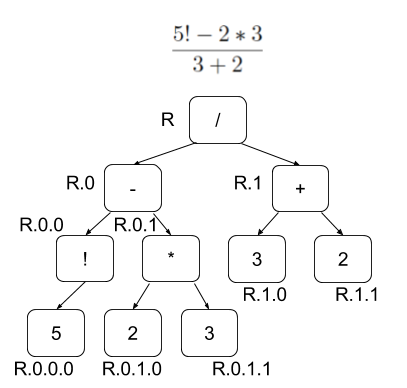
\includegraphics[width=.6\textwidth]{image/Parse_Trees.png}
   \caption{The parse tree mark each tree node by position. "R" stands for root node, "0" stands for left child node and "1" stands for right child node. Therefore, "R.0.1" stands for the right child node of the root's left child.}
   \label{fig:parse_tree}
\end{figure}

To figure out the mistake in an attempt, we compare the parse tree of the attempt with the parse tree of the correct answer. The tree comparison can tell us the subexpression that students make mistakes on. We can then classify student inputs based on the incorrect subexpressions and assign hints correspondingly. For example, the student who typed $5!-2*3$ and the student who typed $\frac{5!-2*3}{10}$ for a problem with solution $\frac{5!-2*3}{3+2}$, as in Fig. \ref{fig:parse_tree}, would be classified as the same group. Both of the students will have a mismatch of tree node $R.1$. This tells the system that the subtree of $R.1$ is wrong and the system will look for the corresponding hint.

One problem is that there are many different ways to write the same math expression. For example, $5!$ can also be written as $5*4*3*2*1$ or $5*4*3*2$. Therefore, we evaluate each subtree and use it in our comparison. The parse trees are evaluated bottom up. The operators at the bottom of the trees are evaluated first. The root operator is evaluated last. See Fig. \ref{fig:eval_tree}. 

Both the parse tree and the evaluation tree are used when we compare the attempt to the correct answer. We identify a subtree as incorrect only when the evaluation and the subtree itself don't match. Therefore, $5!$ and $5*4*3*2*1$ will be identified as the same subtree because it evaluates to the same result.

\begin{figure}[ht]
   \centering
   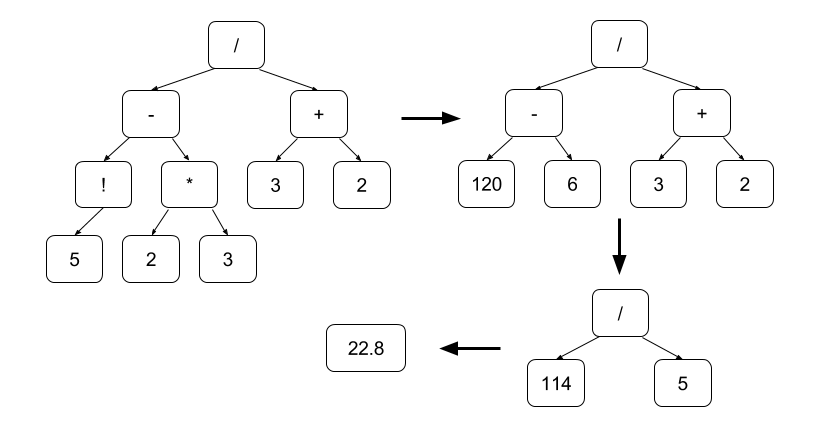
\includegraphics[width=0.8\textwidth]{image/Eval_Trees.png}
   \caption{The parse tree is evaluated bottom up. We first evaluate the lowest level of the tree then pass the evaluated results to the level above. Then use the lower level results to evaluate the upper level of the tree until we reach the top node of the tree, the root, which will give us the final numerical result of the expression.}
   \label{fig:eval_tree}
\end{figure}


\subsection*{Assign Hints}
When TAs create hints, they are also asked to specify rules. Hint rules tell the system when to send certain hints and who the hints will go to. One example of hint rule for expression in Fig. \ref{fig:parse_tree} could be "$R.0.0$ is wrong" and the corresponding hint could be "You need to find the number of ways to arrange 5 poker cards. How many ways can you arrange three different cards?". When the hint system captures an attempt with an incorrect $R.0.0$ subtree, this hint will be sent. Such attempts could be $\frac{4!-2*3}{3+2}$ or $\frac{30-2*3}{3+2}$. The adaptive hint system will assign hints automatically based on the hint rules. This allows our hints to be sent automatically.

Note that the system doesn't send hints to every student. We only send hints to students who have been working on the problem for more than 5 minutes or students who did more than three attempts. We think these students are the ones who are working on the problem actively and are struggling. Furthermore, students need to demand for hints by clicking a "Show Hints" button. Once a hint is assigned to a student, the student can choose to click or not click the "Show Hint" button. One can ignore the assigned hint by not clicking the "Show Hint" button. If a student wants to see the assigned hint, he/she needs to click the "Show Hint" button to see the hint. See Fig. \ref{fig:show_hint} In other words, we only show hints to students who ask for hints. Students who don't click the "Show Hints" button will not see the assigned hints. This makes sure we give hints to students who need helps and actively ask for help. 

\begin{figure}[ht]
   \centering
   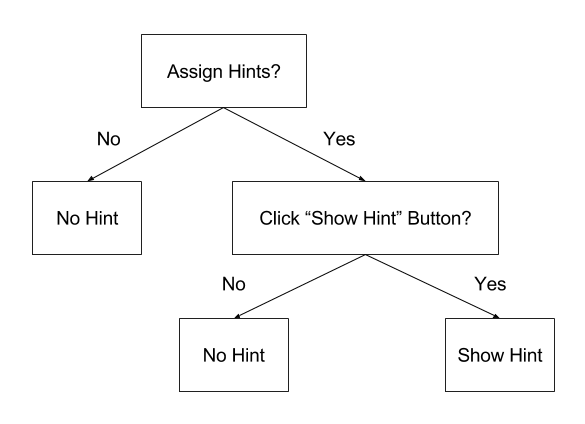
\includegraphics[width=0.6\textwidth]{image/Show_Hint.png}
   \caption{First the system decides whether to assign hints to a student. Then the student gets to decide whether to see the assigned hint. A student will see a hint only if the system decides to assign the hint and also the student decides to see the hint.}
   \label{fig:show_hint}
\end{figure}


\section{Statistical Study on Effectiveness of hints}
The hint system has recorded all the student attempts and the timestamps of each attempt. This allows us to extract useful features, including the number of attempts on each problem, time spent on each problem, etc. These features are used to study what effects hints make on students behavior.

To study the effectiveness of the hint system, we randomly split students into two groups for each assignment, one group with hints(the hint group) and one group without hint(the no-hint group). Each student has 50\% chance of getting a hint on each assignment. If a student is chosen to receive hints on one assignment, he/she will be able to receive hints on all the problems in that assignment. Note that students can still choose not to see the hint on certain problems by not clicking the "Show Hint" button. Therefore, for the students in the hint group, we have two different types of problems. One is \textbf{problems with hints}, these are the problems that students decided to click "Show Hint" to see the hint content. We also have \textbf{problems without hint}, these are problems that students decided not to click the "Show Hint" button. Also, for each problem, we have three groups of students. We first have \textbf{no-hint group}, the group of students receives no hint on the problem. We also have \textbf{hint group}, the group of students receive hints on the problem and clicked "Show Hint" to see the hint content. Finally, we have \textbf{no-show group} the group of students receive hints on the problem but decided not to see the hints by not clicking the "Show Hint" button.

\subsection{Effect on Problems with Hints}
We first look at problems with hints. These problems have at least one hint sent out to at least one student. We extracted the number of attempts students spent on these problems. We calculated the number of attempts for each problem average over students in the no-hint group, and also the number of attempts for each problem average over students in the hint group. We compared these two numbers for each problem and found that students without hint spend fewer attempts on a problem compared to students with hints. See the left graph in Fig. \ref{fig:tries_times_analysis}. This shows that students in the hint group are students who struggle with these problems.

We also extracted the time students spent on each problem. We measured the time differences between each attempt and filtered those that are longer than 10 minutes. We consider the time gaps larger than 10 minutes as students taking a break. We then sum all the time gaps and consider the sum as the total time students spent on the homework problems. We get a similar result comparing to the number of attempts experiment. See the graph on the right of Fig. \ref{fig:tries_times_analysis}. The students with hints spent more time working on problems than the students with no hint. The result is consistent with the number of attempts measurement.

\begin{figure}[ht]
\centering
   \begin{tabular}{c c}
		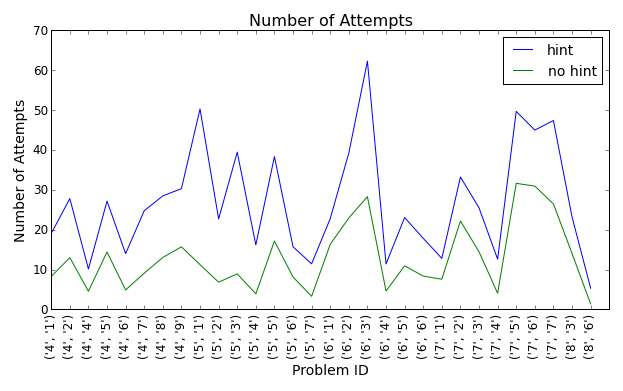
\includegraphics[width=0.5\textwidth]{image/tries_analysis.png} &
		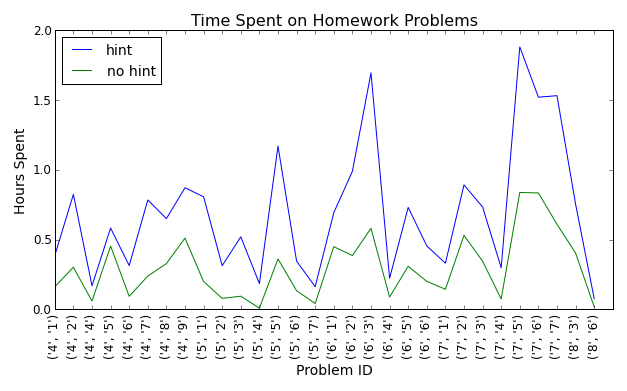
\includegraphics[width=0.5\textwidth]{image/times_analysis.png}
	\end{tabular}
    \caption{On the left, the graph shows number of attempts for each problem average over all students. These problems are problems that at least one student received hints on. It shows that students who ask for hints spent more attempts on these problems than the students in the no-hint group. On the right is the graph of time spent on each problem average over all students in hint group vs. students in no-hint group. Students with hints spend more time on problems than the students in no-hint group. It is consistent with the graph of number of attempts.}
    \label{fig:tries_times_analysis}
\end{figure}

Furthermore, we want to examine whether these two groups of students are significantly different. We performed a two-tailed t-test for both the average number of attempts and the average time spent on each problem. Our null hypothesis was that students from these two groups should have no different on the average number of attempts and average time spent. We found that students who ask for hints spent more attempts on average than students with no hints with a p-value $2.48*10^{-41}$. And students who ask for hints spent more time also with a p-value $6.63*10^{-36}$. We reject the hypothesis and conclude that these two groups of students are significantly different. Students who ask for hints are students who struggle with their homework. They spend more time and more attempts on these problems compared to other students.

Note that students with hints are likely to spend more time on these problems than the students with no hint because all our hints are short questions designed for students to answer. Students will spend time to do the hint questions in between the attempts on the homework problems.

\subsection{Effect on Problems without Hint}
We then look at problems without hints. Our goal is to select the problems with no hint and examine whether adaptive hints help students learn to solve similar problems when no hint is present.

We filtered out the problems that students attempted before the first hint in each homework assignment. We make sure to only look at problems that students solve after they see their first hint. This makes sure students received at least one hint before solving these problems. For example, student A does an assignment of 9 problems in the following order $\{ 1, 4, 3, 2, 6, 5, 7, 8, 9\}$. Student $A$ receive hints on problem $\{3, 5, 7\}$. We will then only look at problem $\{2, 6, 8, 9\}$ in this assignment. We made sure that student A does problem $\{2, 6, 8, 9\}$ after receiving at least one hint in this assignment.

To measure the difference between the hint group and the no-hint group, we first take all the students in the no-hint group and calculate the average number of attempts $t_i$ on each problem $i$. We use $t_i$ as our baseline for each problem $i$. Then for each student in the hint group, we find the problems without hints and sum up all the attempts $s_i$ on these problems. For previous example of student $A$, we would have $S_A = s_2 + s_6 + s_8 + s_9$. We would also have the sum of number of attempts from our baseline $T_A = t_2 + t_6 + t_8 + t_9$. We then compare $S_A$ and $T_A$ to see whether they are the same. See Figure. \ref{fig:pro_no_hint}.

\begin{figure}[ht]
   \centering
   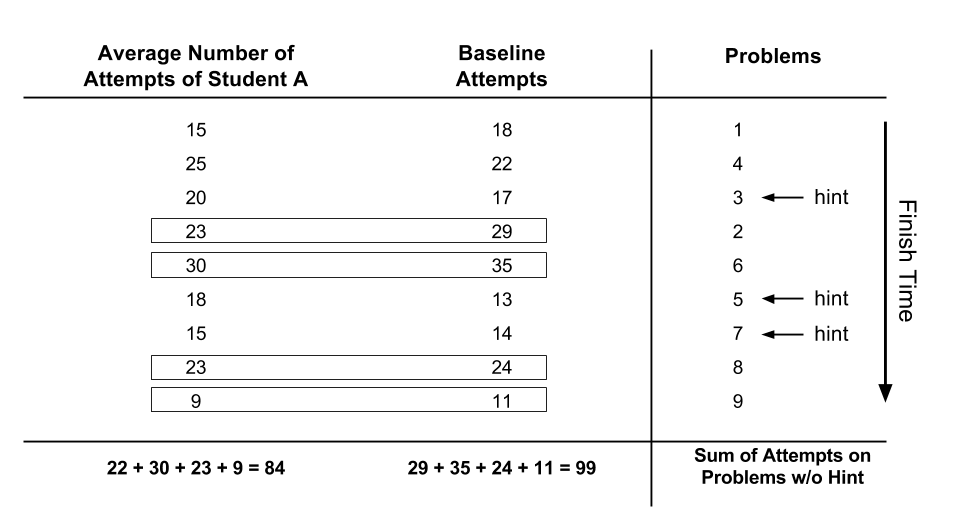
\includegraphics[width=0.8\textwidth]{image/Filter_problems.png}
   \caption{We filter out the problems that come before the first problem with hints. We only look at problems that come after problem 3 in the above example. We then sum up the attempts and compare the sum of attempts for student A and our baseline.}
   \label{fig:pro_no_hint}
\end{figure}



\begin{table}
\caption{The table listed the average extra number of attempts that no-hint group spent than hint group. We first compare the attempts for each assignment, then we look at all assignments at the end. We also perform a two tailed t-test with the null hypothesis that students in no-hint group should have the same amount of attempts on problems as students in the hint group. The final p-value of the two tailed t-test for all assignments is small enough that we can reject the null hypothesis.}

\begin{center}
  \begin{tabular}{| c | c | c |}
  \hline
   Week & Number of attempts of & P-Value \\
      & (no-hint group) - (hint group)  & \\ \hline
	4 & -1.051 & 0.829 \\
	5 & 14.559 & 0.00032 \\
	6 & 5.528 & 0.104 \\
	7 & 14.597 & 0.030 \\
	8 & -1.526 & 0.609 \\ \hline
    All Assignments & 14.409 & 0.029 \\ 
    \hline
  \end{tabular}
  \label{tab:no_hint}
  \end{center}
\end{table}

Our data shows that students in the hint group spend an average of 14.409 fewer attempts than the students in the no-hint group over all assignments. We again perform a two-tailed t-test. Our null hypothesis of our t-test is that students in the hint group should have the similar sum of attempts with students in the no-hint group. The p-value of our t-test is $2.9\%$. Therefore, we reject the null hypothesis and conclude that student performance in the hint group and the no-hint group are significantly different. We concluded that the adaptive hint system helps students to learn to solve similar problems that come later in the assignment. See Table \ref{tab:no_hint}.

Table \ref{tab:no_hint} also shows data for each assignment. Assignment of week 4 and week 8 with very high p-value give negative results, but the results from week 5, 6, and 7 with very small p-value dominate the final result for all assignment. Let's look at week 4 and week 8 in detail. If we look at week 8, we found that there are only 176 hints sent. Therefore, the data we collected for week 8 may not be enough for us to detect the difference between two groups of students. If we look at week 4 in detail, we found that out of a total of 9 problems in week 4 assignment, problem 5 has 549 hints received and problem 9 has 96 hints received. The rest of the problems all have less than 50 hints received by students. This may cause the data to be too biased and therefore lead to a very large p-value. Week 4 is the first week we started to send hints to students and students could still be in the process of learning how to request hints and how to learn from hints.

As a conclusion, the result shows us that the adaptive hints help students to learn to solve problems and as a result improve students' performance in homework. Students who learn from hints perform better on similar problems comparing to students without hints.

\section{Conclusion}


\newpage
\bibliographystyle{splncs}
\bibliography{bibtxt}



\end{document}e